%\KZ{This section doesn't quite stand by itself, %because this is not really a dataset paper.
%The word ``Dataset'' implies that the data will be %shared and reused by other people.
%I don't think this is the case here? We just wanna %tell them the results from analyzing the data;
%we might not want to release the data itself, due to %privacy concerns?
%I think part of this section should go into the %approach section, and part of it should go into
%the results section.}

\section{Experiments and Analysis}
\label{sec:results}
In this section, we conduct two experiments, \textit{target depressed users identification} and \textit{live interaction experiment} with the selected depressed users using different roles. 
%\SY{I didn't see the result of depressed user identification. Do you mean ``we identify target users and analyse their posts''?}
The former is a static analysis of the Weibo data we collected, while the latter aimed at addressing the following three issues: 
1) Do depressed users prefer to interact with chatbots or humans? 
2) What types of roles are depressed users more willing to interact with, 
including ordinary people, psychological counselors, current depressed users, 
or recovered depressed users? 
3) Which response strategy is easier to break the ice for depressed users?
%In this section, we analyze Weibo depression data and address the following three issues:
%\KZ{Actually you are not answering these questions by analyzing the Weibo data, cos that data is a static one,
%which consists of all the users you have crawled from the super %topic; you can only answer these questions through
%a \textbf{live} interactive experiment. This is the most interesting part of this paper!!}

%\KZ{Need to restruct this section into two parts (experiments): depressed user identification, 
%and live interaction with the selected users using different roles. To do the first experiment,
%we first need to collect data (actually this process can be ongoing continuously).}

%\KZ{The results from prev section are also important %analysis, and should be included in this section.
%No need to mention ``Results'' and ``Analysis'' in each %and every subsection headings, cos we know they are
%results and analysis.}
%\begin{enumerate}
	%\item Do depressed users prefer to interact with chatbots or humans?
	%\item What types of roles are depressed %users more willing to interact with, including ordinary people, psychological counselors, current depression users, or recovered depression users?
    %\item Which response strategy is easier %to break the ice for depressed users?
%\end{enumerate}
%\KZ{After these question, you should talk about experiment setup. People are interested in knowing how you conduct these experiments, the scale of the examples, because when you talk about the success rate etc, people want to know
%the size of the support of your experiment, if it has any statistical significance, etc. So you should first talk about
%the experimental setup.}

\subsection{Target Depressed Users Identification}
% \subsubsection{Dataset}
Our Proactive Ice-breaking System monitored the depression super topic community for 60 days and collected information on 2193 individuals with depression.
%\KZ{This section is not only about the stats of the dataset. Change the sec heading.
%The organization and position of this subsection is a bit weird. It's part static analysis and partly relies on the
%interactive experiment. I think you need to re-org this whole section.}
% \subsubsection{Gender Distribution}
We use the depressed user detector in the \secref{sec:depression_detection} to screen out users with depression, and then calculate the gender distribution of depressed.
There are 1695 users with depression, including 216 males (\textbf{12.7\%}) and 1479 females (\textbf{87.3\%}). The number of female depressed users on Weibo is significantly higher than that of males. Studies~\cite{ahmed2023chatbot} have shown that women are more prone to depression. \citet{kuehner2017depression,lu2021prevalence} pointed out that women are more likely to suffer from depression, mainly because of physiological factors such as sex hormone fluctuations, as well as social and psychological factors such as high stressors, low self-esteem, physical shame and experiencing violence.
%\KZ{Any explanation why females turn to social media much more than males? Literature support?}

%\KZ{The following paras are already analysis, and they %should go into the results and analysis section.
%You need to define what is ``success'' before you talk %about success rate.
%The two figs seem to be waste of space as they are be %represented much more succinctly.}
\subsubsection{Key Factors of Ice-breaking Success}
We define ``success'' as completing all three rounds of conversations with a depressed user, and we analyze the key factors affecting the success rate of ice-breaking as follows.
\paragraph{Gender}
On social media, gender differences among users with depression may affect the success rate 
of ice-breaking. The success rate here is the proportion of posts that have successfully conducted three rounds of interactions (ice-breaking success) under a certain gender, as shown in Formula\ref{eq:gender}. As shown in~\figref{fig:success_gender}, the success rate of female users in ice-breaking is higher than that of males.

\begin{equation}
    P(\text{positive} \mid \text{gender}) = \frac{N(\text{positive, gender})}{N_{\text{total}}}
    \label{eq:gender}
\end{equation}
\noindent
where $P (positive | gender)$ represents the probability of ice-breaking success posts given a specific gender, $N(positive, gender)$ is the number of ice-breaking success posts made by users of a specific gender,  $N_{total}$ is the total number of posts made by all users, regardless of gender.

\begin{figure}[th]
    \centering
    \includegraphics[width=0.7\columnwidth]{images/success_gender.png}
    \caption{Success rate between the genders.}
%\KZ{Sucess rate is the number of successful ice-breaking attempts over all ice-breaking attempts.}
%For reference, success rate is calculated... \MY{please %maker sure the fonts in your figures are consistent, also %they should have bigger font size, including the legend. %same for the following figures} \KZ{Pls define
%success rate also. Is it number of successes over number %of attempts?}
    \label{fig:success_gender}
\end{figure}

\paragraph{Density}
Density refers to the average number of posts posted by depressed users every day (under the posts obtained), as shown in \eqref{eq:density}. The historical posting density of users reflects the stickiness of user's use of social media to a certain extent.
According to the user post density, the change of ice-breaking success rate is shown in \figref{fig:success_density}. The success rate here is the proportion of posts that successfully engage in three rounds of interaction (ice-breaking success) at a certain density, as shown in the Formula \ref{eq:density_success_rate}.
When the posting density falls on (4,50], the broken success rate is the highest, while when the posting density falls on (0.05,0.1], the broken success rate is the lowest.
The higher the density of user posts, the more frequent they are posted, and the easier it is for chatbot to break the ice with them.

\begin{equation}
    D_{\text{posts}} = \frac{N_{\text{posts}}}{T}
    \label{eq:density}
\end{equation}
\noindent
where N\text{posts} is the number of posts posted during time period T, and T is the number of days in the time period.

\begin{equation}
    P(\text{positive} \mid D_{\text{posts}}) = \frac{N(\text{positive, density})}{N_{\text{total}}}
    \label{eq:density_success_rate}
\end{equation}
\noindent
where $P (\text{positive} | D_\text{posts})$ represents the proportion of positive posts under a certain post density. $N(\text{positive, density})$ is the number of positive posts under a certain post density. N\text{total} is the total number of all posts.

\begin{figure}[th]
    \centering
    \includegraphics[width=1\columnwidth]{images/success_density.png}
    \caption{Ice-breaking success rate by user post density.}
    \label{fig:success_density}
\end{figure}

%\KZ{You might want to have a summary (in bullet form) %that summarizes the findings above?}

\subsubsection{Post and Reply Category Proportions in Positive Samples}
To determine whether the categories of posts and replies will affect the success rate of ice breaking, we analyze the proportion of each category under ice-breaking success posts and replies. The calculation formula is shown in Formula \ref{eq:post_reply}.

\begin{equation}
    P_{\text{category, positive}} = \frac{N_{\text{post~|~reply, positive}}}{N_{\text{total, positive}}}
    \label{eq:post_reply}
\end{equation}
\noindent
where $P_{\text{category, positive}}$ represents the proportion of a specific category (post or reply) in positive samples, and $N_{\text{post | reply, positive}}$ is the number of a specific category (post or reply) within positive samples, and N{\text{total, positive}} is the total number of that category (post or reply) in positive samples.

\paragraph{Post Categories}
%According to the statistics of different categories of posts, as shown in ~\figref{fig:success_post}, matter what kind of posts, the proportion is above 0.6, and the difference is not big, indicating that the post category has little to do with the success rate of ice-breaking.
 According to the statistics of different categories of posts shown in \figref{fig:success_post}, the proportion of successful interactions is above 0.6 for all post categories, with little variation. This indicates that the post category has little impact on the success rate of ice-breaking.
%\SY{I rewrite this: According to the statistics of different categories of posts shown in \figref{fig:success_post}, the proportion of successful interactions is above 0.6 for all post categories, with little variation. This indicates that the post category has little impact on the success rate of ice-breaking.}
%\KZ{Why are the success rates of men are women
%both below 0.5 while the success rate of these post categories are %all above 0.6? Something
%is not right? Do you have a diff definition of success rate for %each of these 
%experiments?}

\begin{figure}[th]
    \centering
    \includegraphics[width=1\columnwidth]{images/success_post.png}
    \caption{Proportion of post categories under positive samples.}
    \label{fig:success_post}
\end{figure}

\paragraph{Reply Categories}
As shown in~\figref{fig:success_reply}, the ice-breaking success rate is highest when the reply category is ``Suggestions and Solutions'', and lowest when the reply category is ``Negative Reply''.

\begin{figure}[th]
    \centering
    \includegraphics[width=1\columnwidth]{images/success_reply.png}
    \caption{Proportion of reply categories under positive samples.}
    \label{fig:success_reply}
\end{figure}

\subsection{Live Interaction Experiment}
After our exploration through the dataset above, we now want to answer the research questions we raised earlier. To achieve this, we conducted a live experiment to observe the interactions between depressed users and different factors.
\label{sec:result_chatbot}
\subsubsection{Experiment Settings}
\paragraph{Role Playing}
To address the questions raised above, we created eight different accounts for role-playing as humans and chatbots. The four roles we created are \textit{normal people}, \textit{psychological counselor}, \textit{current depressed user}, and \textit{recovered depressed user}. Both humans and chatbots were assigned these four different roles.

For humans, the variation in account identity was primarily achieved through different followers and post histories. The normal role featured life-sharing posts and an overall positive attitude, while the depressed roles had many historical posts with a negative tone. For the psychological counselor role, we named the account ``Psychological Counselor XXX'' and mentioned that the user is a certified counselor in the profile introduction. Additionally, the post histories for this role included mental health-related content, offering advice and suggestions.

For the chatbot accounts, the identity was established through the account name, profile picture, and profile introduction. We included ``bot'' in the account name and provided different identifiers before the word ``bot''. We also used chatbot-like profile pictures and clearly stated in the profile that they are chatbots. \figref{fig:roleplay} shows an example of the account profile.
\begin{figure}[th]
    \centering
    \includegraphics[width=1\columnwidth]{images/roleplay3.png}
    \caption{Example of the account profile for roles.The upper profile is for the Human-Recovered Depressed users role, the middle profile is for the Human-Ordinary People role, while the lower profile is for the Chatbot-Current Depressed users role.}
    \label{fig:roleplay}
\end{figure}

\paragraph{Dataset}We selected 800 posts from posts that are easy to break for comments, and each of the eight accounts replied to 100 posts. We collected data on whether the users responded to our replies and what their responses were.
%Additionally, we recruited one volunteer to evaluate the strategies used in each reply.
\ZT{Additionally, we recruited a volunteer to review each reply for its appropriateness to the specified role and strategy. Given that this is a simple task, this native Chinese-speaking volunteer with a university education background is sufficiently qualified for the task.}

\begin{table*}[th]
	\small
    \centering
	\begin{tabular}{p{0.35\columnwidth}|p{0.3\columnwidth}|p{0.3\columnwidth}|p{0.3\columnwidth}|p{0.3\columnwidth}|p{0.2\columnwidth}}
		\toprule
		\diagbox{Role}{strategy} & {Emotional support \( \mbox{\&} \) resonance} & {Suggestions  \( \mbox{\&} \) solutions} & {Emotional talk \( \mbox{\&} \)
 communication} & {Encouragement  \( \mbox{\&} \) affirmation} & {All}\\ \midrule
		Ordinary users & 0.19 / 0.38 & 0.13 / 0.39 & 0.06 / 0.38 & 0.18 / 0.24 & 0.15 / 0.35 \\ \midrule
		Counselors & 0.16 / 0.24 & 0.17 / 0.32 & 0.11 / 0.08 & 0.31 / 0.13 & 0.25 / 0.21   \\ \midrule
        Current depressed users & 0.27 / 0.27  & 0.31 / 0.33 & 0.06 / 0.31 & 0.38 / 0.25 & 0.28  / 0.28  \\ \midrule
        Recovered depressed users & 0.27 / 0.34 & 0.29 / 0.58 & 0.50 / 0.48 & 0.36 / 0.19 & \textcolor{red}{\textbf{0.34}} / \textcolor{blue}{\textbf{0.41}}  \\ \midrule
        All & 0.23 / 0.34 & 0.26 / \textcolor{blue}{\textbf{0.38}} & 0.20 / 0.37 & \textcolor{red}{\textbf{0.30}} / 0.20 &  \ 0.26 / \textbf{0.31}  \\ \midrule
	\end{tabular}
	\caption{Success rate of chatbot / human roles. The success rate is calculated as described in \secref{sec:result_interaction}. The red and blue bold parts in the table represent the best performance of chatbot and human in role and strategy respectively, and the black bold part represents the highest total success rate of human.}%\KZ{What are the numbers in the table?
%Success rate? Pls say it clearly. Shouldn't the total on the right be the sum of
%every row's numbers? Now it's more like an average.
%These two tables are too loose. Try to remove the white space
%and maybe make them two narrow tables.}\MY{Total is actually average? What's the difference between emotion support resonance and emotional talk communication?}
	\label{tab:response_result}
\end{table*}

%\begin{table*}[th]
%	\small
 %   \centering
%	\begin{tabular}{p{0.35\columnwidth}|p{0.3\columnwidth}|p{0.3\columnwidth}|p{0.3\columnwidth}|p{0.3\columnwidth}|p{0.2\columnwidth}}
%		\toprule
%		\diagbox{Role}{strategy} & {Emotional support and resonance} & {Suggestions and solutions} & {Emotional talk and communication} & {Encouragement and affirmation} & {Total}\\ \midrule
%%		ordinary people & 0.44 & 0.5 & 0.31 & 0.28 & 0.34 \\ \midrule
%		psychological counselors & 0.24 & 0.31 & 0 & 0.09 & 0.19   \\ \midrule
 %       current depression users & 0.25 & 0.2 & 0.42 & 0.27 & 0.27   \\ \midrule
  %      recovered depression users & 0.34 & 0.72 & 0.44 & 0.24 & \textbf{0.4}   \\ \midrule
   %     Total & 0.33 & \textbf{0.38} & 0.37 & 0.22 &    \\ \midrule
	%\end{tabular}
	%\caption{User success result of human.}
	%\label{tab:human_strategy_result}
%\end{table*} 

\subsubsection{Results}
\label{sec:result_interaction}
 We calculated the success rate by dividing the number of user responses for a specific role \textbf{and} strategy by the number of icebreakers sent for that role \textbf{and} strategy. The total success rate is calculated by dividing the number of user responses for a role \textbf{or} strategy by the total number of icebreakers sent for that role \textbf{or} strategy. The success rate results can be seen in~\tabref{tab:response_result}. With these results, we answered the three questions mentioned earlier.

\paragraph{Chatbot vs. Human}
Research has shown that compared to face-to-face chatting with humans, communicating with emotional chatbots can reduce negative emotions and concerns, and people are more willing to communicate with chatbots ~\cite{drouin2022chatting}.
However, as shown in~\tabref{tab:response_result}, the number of replies to humans (0.31) is higher than that to chatbots (0.26). When humans do not express negative emotions, show respect for depressed users, and choose appropriate strategies to communicate, depressed users are more willing to interact with them.
\ZT{Notably, human icebreakers do not always outperform bots. When taking on the role of current depressed users, the ice-breaking success rate of humans and bots is the same. When taking on the role of counselors, bots have a higher ice-breaking success rate than humans. The aim of this study is to discover which strategies used by icebreakers are more preferred by depressed users on Weibo, and whether depressed users prefer to interact with human or bot icebreakers. Therefore, despite the overall higher willingness of depressed users to engage with human icebreakers, the value of this study is still reflected.}

\paragraph{Role Preference}
~\tabref{tab:response_result} indicates that, whether chatbots or humans, users who play the role of a recovered depressed user have the highest success rate (chatbot: 0.34 / human: 0.41). This shows that depressed users are more willing to interact with users who have recovered from depression. One probable reason is that individuals with depression can relate to the recovered-depression user, feeling encouraged by their success in overcoming the illness, and trust that they can provide valuable suggestions, making them more willing to respond.
However, other roles are ranked differently. Ordinary users rank last when played by chatbots (0.15), possibly because these chatbots' responses are more rigid and lack empathy, causing users to feel it's not worth their time to interact with them. For human roles, ordinary people rank second (0.35), followed by current depressed users (0.28) and counselors (0.21). This may be because ordinary people tend to have a more positive attitude than current depressed users, making the depressed users more willing to respond to them. Counselors received the lowest success rate, possibly because Weibo is a social media platform where all responses are public, and depressed users may not want to disclose too much about themselves. Additionally, depressed users might be uncertain about the professionalism of the Counselors.

\paragraph{Ice-breaking Strategy Preference}
~\tabref{tab:response_result} shows the effectiveness of different ice-breaking strategies. For chatbot roles, encouragement and affirmation ranked the highest (0.30), followed by suggestions and solutions (0.26), emotional support and resonance (0.23), and emotional talk and communication (0.20). This may be because depressed users are more accustomed to hearing encouragement and affirmation from chatbots, while they may not find a chatbot's words of emotional talk and communication credible. For human roles, however, suggestions and solutions ranked the highest (0.38), followed by emotional talk and communication (0.37), emotional support and resonance (0.34), and encouragement and affirmation (0.20). This may be because depressed users find the suggestions particularly relevant and applicable to their own situations.

\paragraph{Case Study}

The responses we received varied. Some responses were contextually related to the icebreakers, especially those employing emotional support \( \mbox{\&} \) resonance and emotional talk \( \mbox{\&} \) communication strategies. Examples include, ``\textit{That's great, being happy, eating delicious food, and learning about things you're interested in. Not bad, very good [Haha][Haha],}'' and ``\textit{Yes [Tear] Sweet like a little bun [Tear].}'' Other responses expressed gratitude or provided emotional support, such as ``\textit{Thank you [Tear][Tear] Keep it up [Effort][Hug][Hug]},'' ``\textit{Hug you,}'' and ``\textit{Yes!}'' Notably, there were no discouraging responses or criticisms.

\figref{fig:case1} shows an example of ice-breaking. The depressed user mentioned that she has decided to live well and try to save herself. Both human and a chatbot replied to this post. The human roles were a recovered depressed user and a normal person, while the chatbot played the role of a current depressed user. The human recovered depressed user employed the strategy of emotional talk and communication, whereas both the normal human and the current depressed chatbot used the strategy of encouragement and affirmation. Interestingly, both human roles received a response from the user, while the chatbot role did not receive any reactions.

This case shows that depressed users are more willing to interact with humans than with chatbots. Among the human roles, the recovered depressed user, who used the emotional talk and communication strategy, received a faster response than the normal human with the encouragement and affirmation strategy. This observation aligns with our previous findings.

\begin{figure}[th]
    \centering
    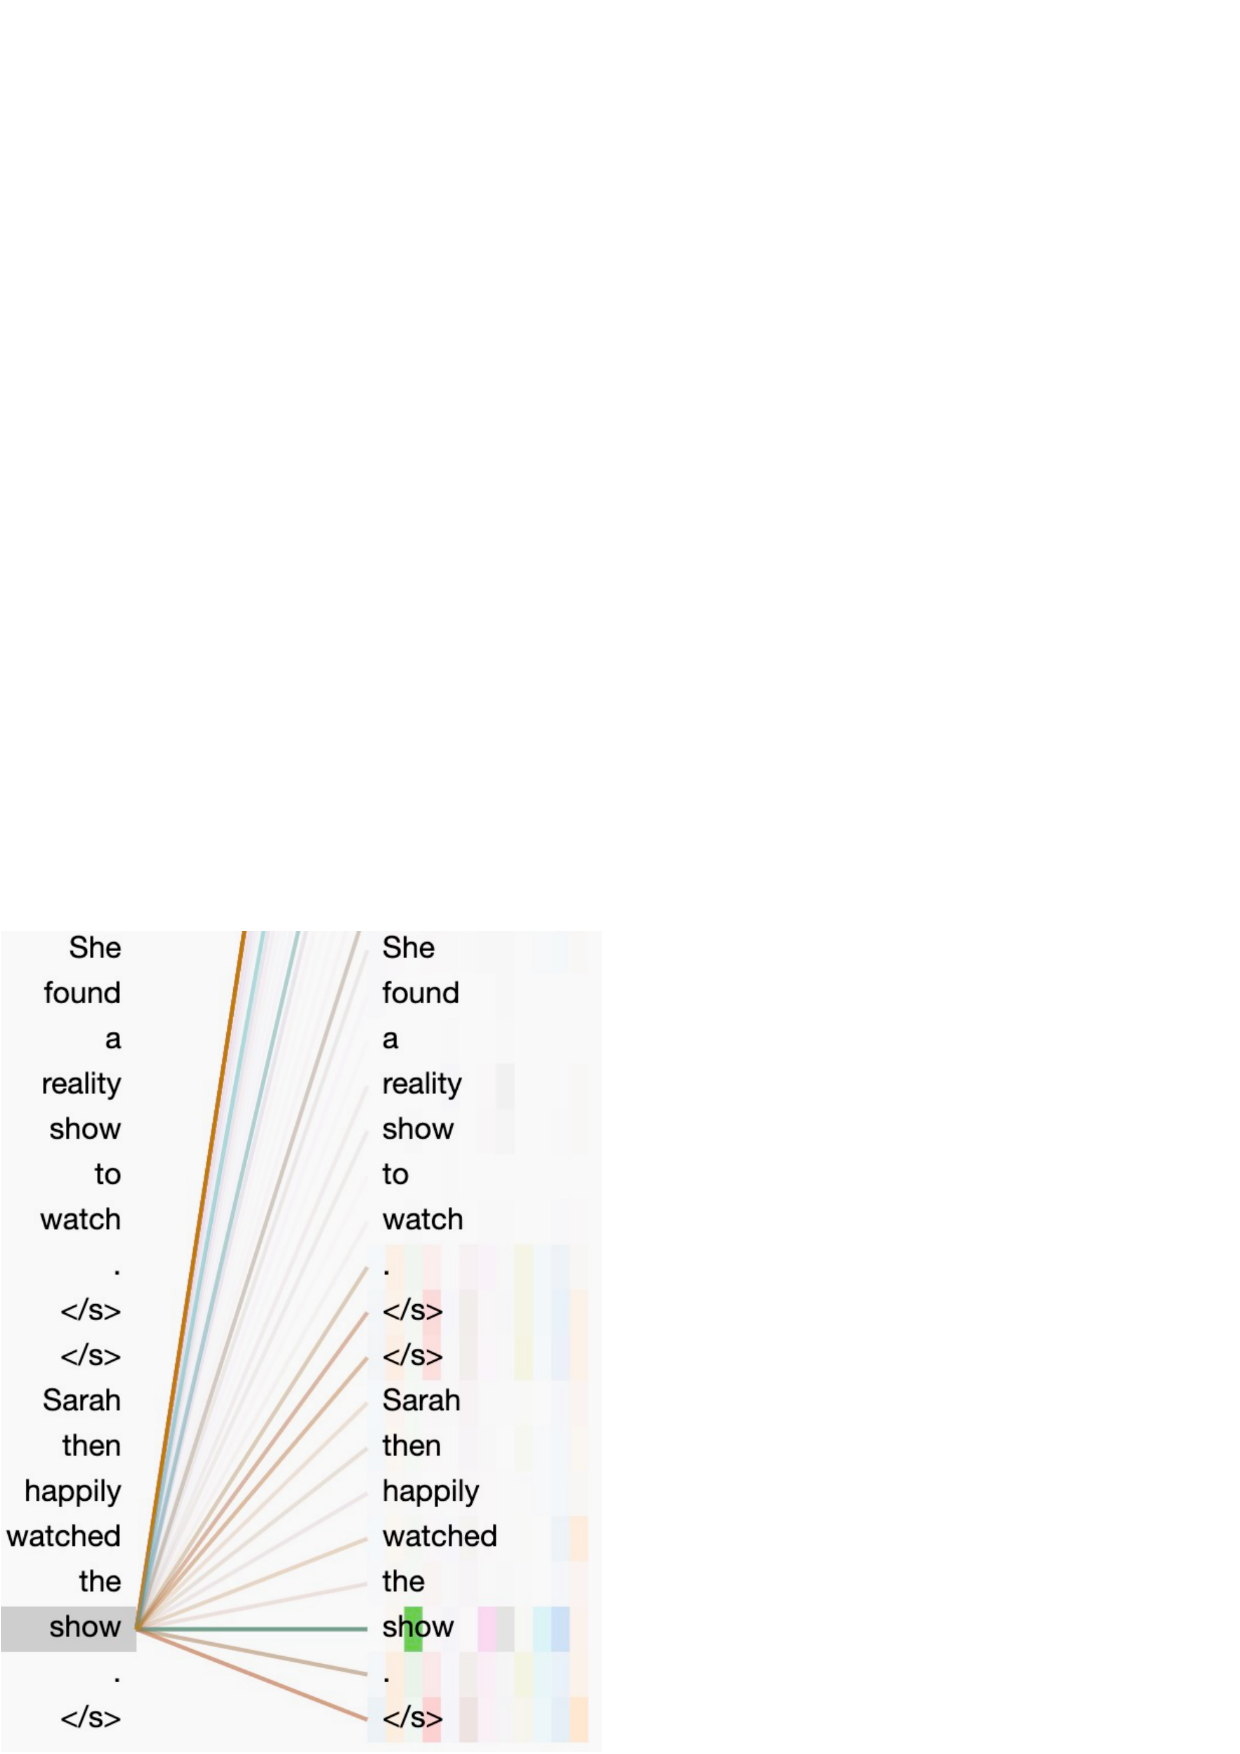
\includegraphics[width=1\columnwidth]{images/case.jpeg}
    \caption{Case Study of an ice-breaking between the depressed user and three different roles.}
    \label{fig:case1}
\end{figure}

